\documentclass{beamer}
\usepackage[utf8]{inputenc}
% \usepackage{polski}
% \usepackage[polish]{babel}
\usepackage[T1]{fontenc}
\usepackage{tikz}
\usepackage{tikzducks}
% \usetikzlibrary{decorations.pathmorphing}
\usepackage{multimedia}
\usepackage{graphicx}
\usepackage[justification=centering]{caption}
\usepackage{textcomp}
\usepackage{appendixnumberbeamer}
\usepackage{qrcode}
% \usepackage[natbib, language=polish, sorting=none]{biblatex}
% \addbibresource{lio.bib}
\usepackage{hyperref}
%\usepackage[width=\textwidth]{animate}
%\usepackage{chemformula}
\usepackage{sidecap}
\usepackage{multirow}
\usepackage{rotating}
\usepackage{anyfontsize} % change font size for semposiwko

\usepackage{physics}

\usepackage{listings}
\lstset{
basicstyle=\small\ttfamily,
columns=flexible,
breaklines=true
}

% \usepackage{emoji}
\usepackage{subcaption}


\usepackage[natbib, language=polish, sorting=none]{biblatex}
\addbibresource{lio.bib}
\renewcommand*{\bibfont}{\scriptsize}

\usefonttheme[onlymath]{serif}

\usetheme{Szeged}
\usecolortheme{whale}
\setbeamercolor{palette primary}{bg=violet!80!black,fg=white}
\setbeamercolor{palette secondary}{bg=violet!60!black,fg=white}
\setbeamercolor{palette tertiary}{bg=violet!40!black,fg=white}
\setbeamercolor{palette quaternary}{bg=violet!20!black,fg=white}
\setbeamercolor{structure}{fg=violet!60!black}
\setbeamertemplate{caption}{\insertcaption}
% \setbeamertemplate{headline}{
%   \begin{beamercolorbox}[wd=.9\paperwidth]{headline}
%     \vspace{1.5ex}
%     \insertsectionnavigationhorizontal
%     \vspace{1.5ex}
%   \end{beamercolorbox}
% }

\linespread{0.6}

\setbeamertemplate{background}%
{%
    \begin{tikzpicture}[remember picture,overlay]{\node[yshift=1.5cm,xshift=-2cm,opacity=0.1] at (current page.south east)
      {
      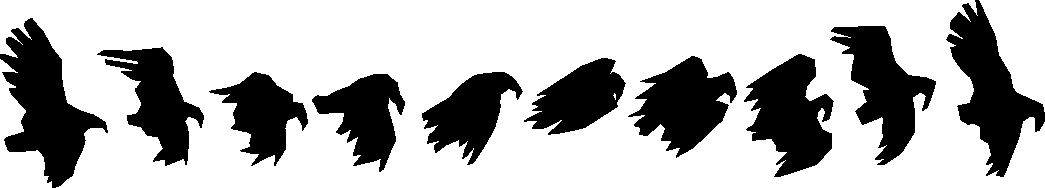
\includegraphics[scale=0.4, angle=20]{ptaki.pdf}
      }
      ;
    \node[yshift=1.0cm,xshift=0.6cm] (logopos) at (current page.south west) {{\begin{tikzpicture}\shuffleducks\duck[signpost=\insertframenumber, \randomhead,scale=.4]\end{tikzpicture}}};
    \pgfmathsetmacro{\progress}{360*(\insertframenumber)/(\inserttotalframenumber)};
    \draw[line width=0.2*3pt] ([xshift=0.55cm] logopos)  arc[radius=0.55cm, start angle=0, end angle=\progress];
    \fill ([shift={(\progress:0.55cm)}] logopos) circle(1pt);

    }
        \end{tikzpicture}
    
}

\newcommand{\SeMPowisko}{%
\large S\normalsize%
\kern-.3em \lower.2ex\hbox{e}%
\lower.2ex\hbox{\large M\normalsize}%
\kern-.1em \raise.1ex\hbox{\large P\normalsize}%
\kern-.3em \lower.2ex\hbox{o}%
\kern-.2em \raise.2ex\hbox{w}%
\lower.2ex\hbox{i}%
s%
\raise.2ex\hbox{k}%
\kern-.3em \lower.2ex\hbox{o}%
}

\newcommand\Tikz{Ti\emph{k}Z}
\definecolor{neworange}{RGB}{255,140,0}


\title{Flywheels}
\subtitle{from zero to wheel}
\author[M. Winiarski]{Mateusz "\(\blacksquare\)" Winiarski}
\institute[Green Energy]{"physics", WFAIS, Jagiellonian University}
\date[dzisiaj]{today}

\begin{document}

\frame{\titlepage}

\section{What are flywheels}

\begin{frame}
\begin{figure}
    \centering
    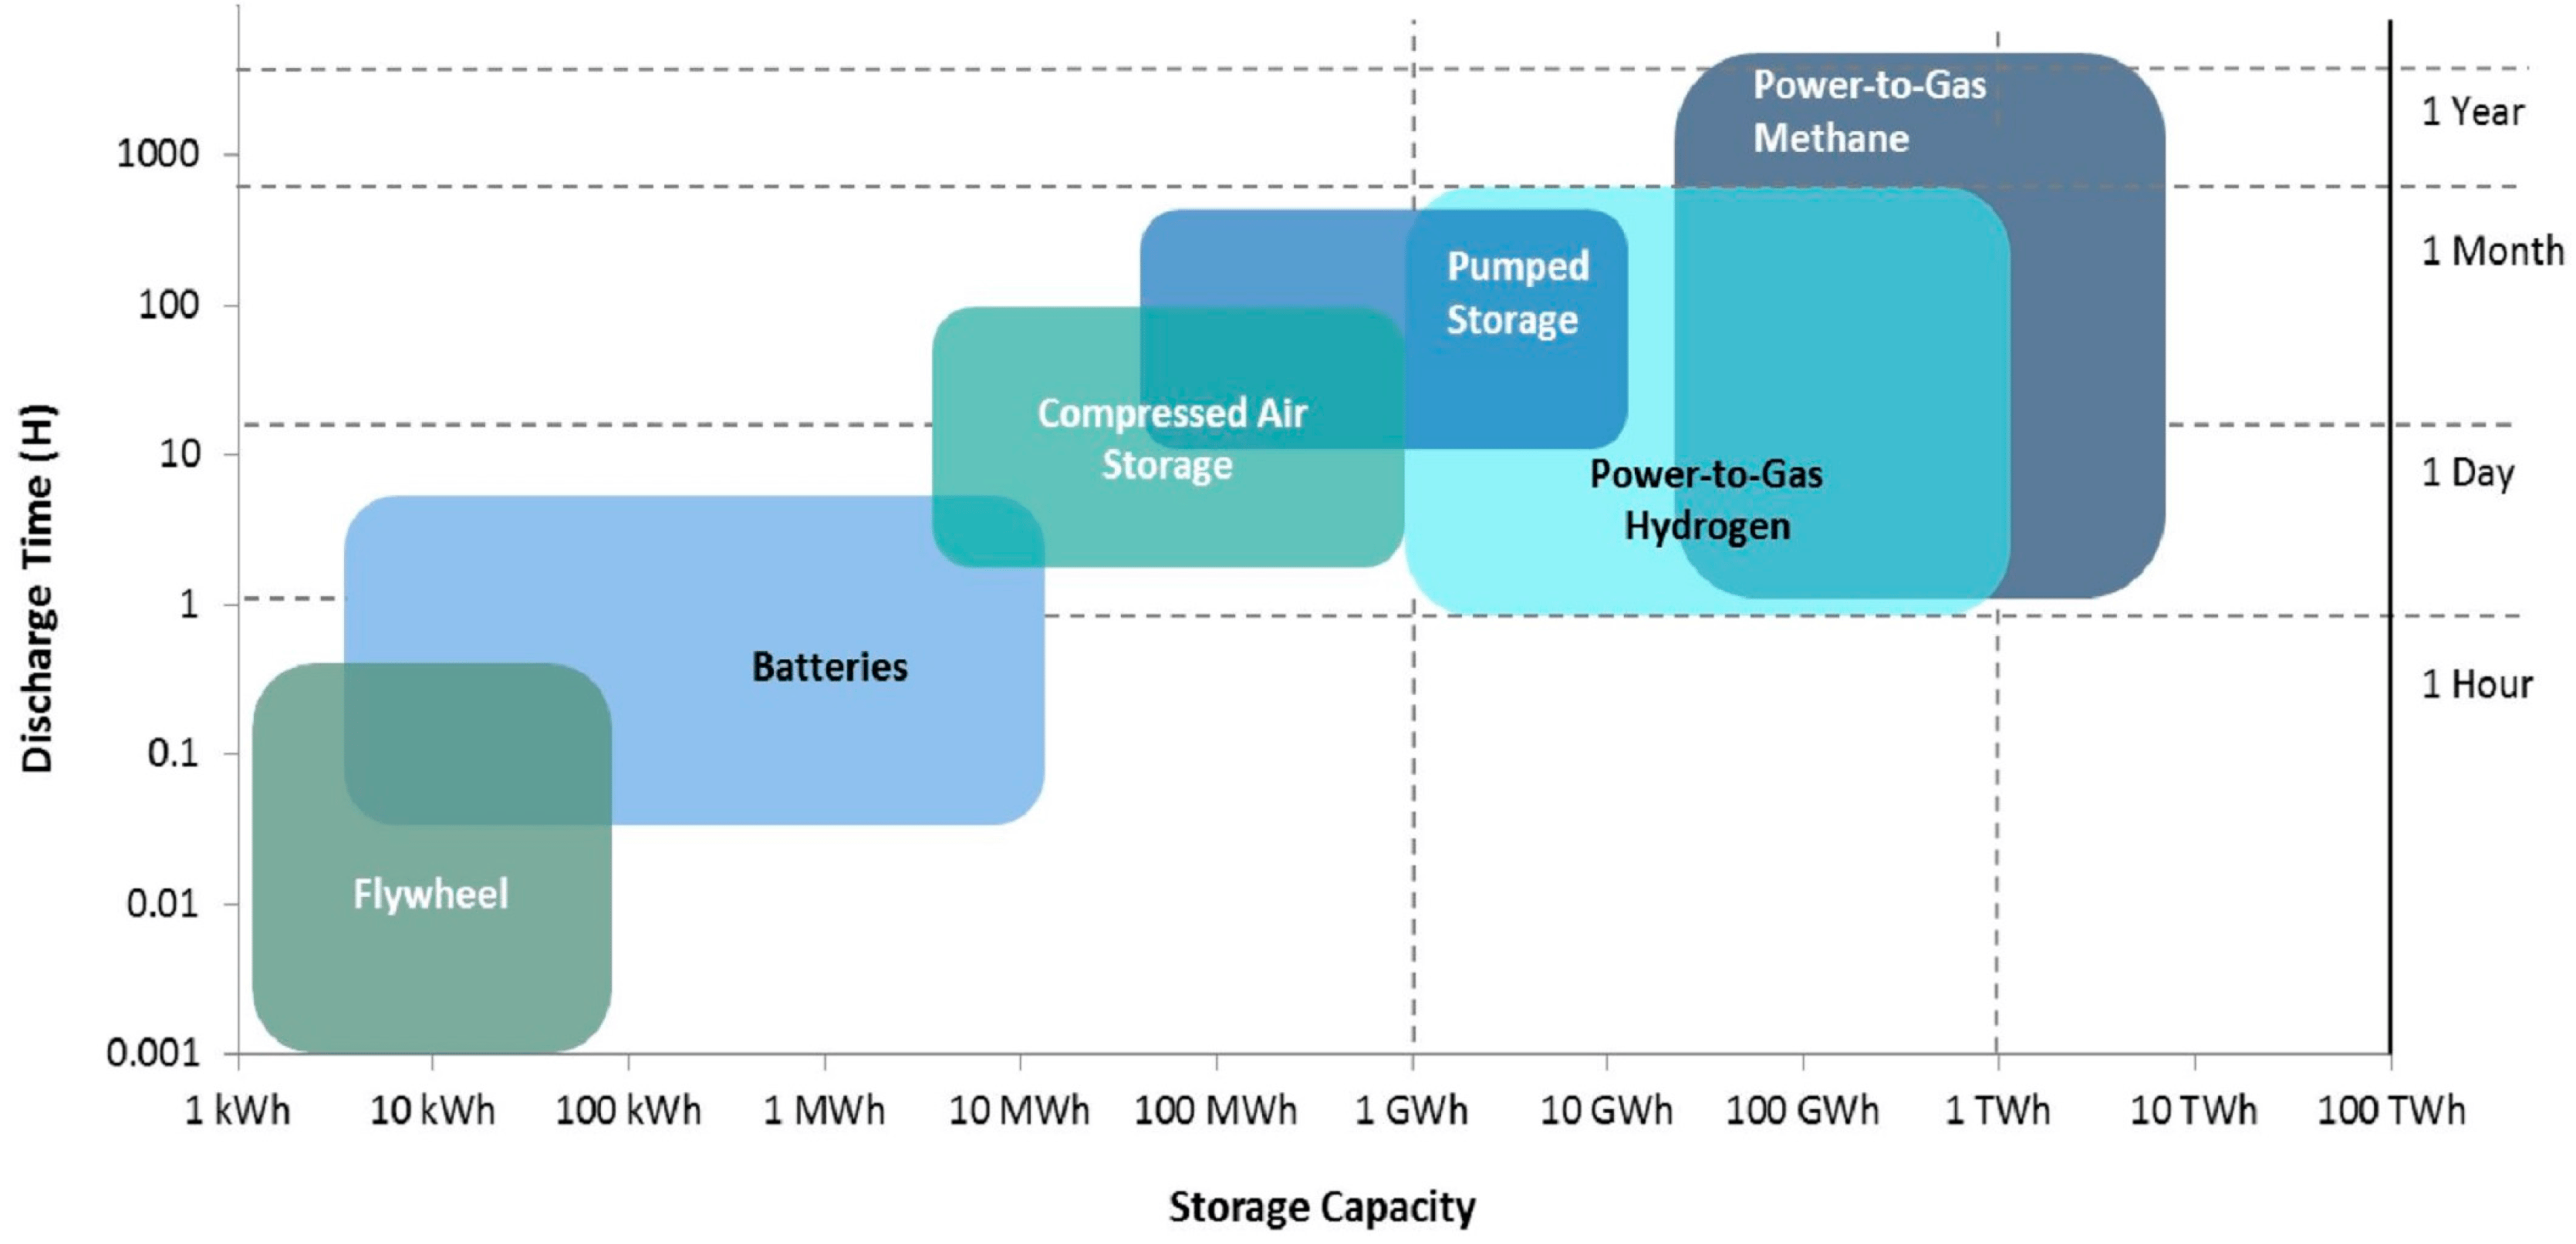
\includegraphics[width=\linewidth]{2025-01-23-00-37-56.png}
    \caption{Comparison of discharge time vs capacity of energy storage technologies (source: \url{doi.org/10.3390/en9090674})}
\end{figure}
\end{frame}

\section{Some math}

\begin{frame}{Physical characteristics}{}
    moment of inertia: \(J=\displaystyle{\int\limits_m} r^2 \dd{m}\)

    % angular velocity: \(\omega = \)

    rotational energy: \(E_{kin}=\displaystyle{\frac12} J \omega^2\)
\end{frame}

\begin{frame}{Specific energy}
    \[\frac{E}{m}=K\frac{\sigma}{\rho}\]

    \begin{itemize}
    \item \(K\) -- shape factor [dimensionless]

    \item \(\sigma\) -- tensile strength [Pa]
    \end{itemize}
\begin{figure}

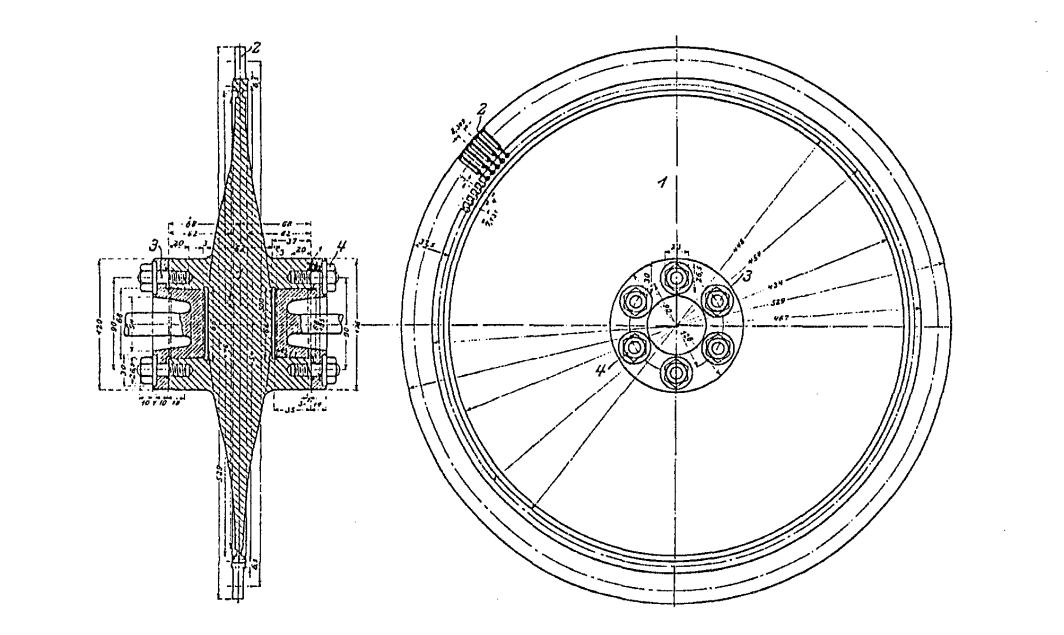
\includegraphics[width=0.6\textwidth]{2025-01-23-16-37-11.png}
\caption{Constant stress turbine disc built by De Laval at the end of XIX century (source: \url{doi.org/10.1007/BF01556455})}
\end{figure}

    % \url{doi.org/10.1109/TIE.2017.2772205}
\end{frame}

\section{Applications}

\begin{frame}{}

\begin{figure}

\centering
    
\begin{tikzpicture}
      \duck[parrot, body=gray!30!yellow, head=gray!30!yellow, bill=red, torch=gray!70!brown, tshirt=white!20!black, strawhat=brown!50!white, ribbon=gray, bowtie=blue!50!white]
      %\addwater{blue!50!cyan}
      \fill[cyan!20!white] (-1.4,1.8) ellipse (1.8 and 0.5);
  \fill[cyan!20!white] (-0.2,1.54) -- (0.2,1.35) -- (0.0,1.6) -- cycle;
	\node at (-1.4,1.8) {thanks for attention};
    \end{tikzpicture}
    \end{figure}


    
    \begin{figure}
    \centering
    \qrcode[height=0.3\textwidth]{https://github.com/falcotinnunculus/przezrocza/blob/wladca/red_energy/flywheel.pdf}\\
    {\tiny \url{https://github.com/falcotinnunculus/przezrocza/blob/wladca/red_energy/flywheel.pdf}}

    \end{figure}
\end{frame}

\end{document}